\mysection{АНАЛИЗ ПРЕДМЕТНОЙ ОБЛАСТИ}
\
\subsection{Машинное обучение. Задача классификации}
\

\textbf{Машинное обучение} – группа методов искусственного интеллекта, которые используются компьютерными системами для эффективного выполнения конкретной задачи без использования явных инструкций, вместо этого обучаясь на множестве решений сходных задач.

Машинное обучение подразделяется на обучение по прецедентам, что означает выявление общих закономерностей на выборке частных данных, и дедуктивное обучение, при котором используется некоторая база знаний, сформированная на основе формализованных знаний экспертов.

В данной работе речь пойдет об обучении по прецедентам, одним из подтипов которого является обучение с учителем. Обучение с учителем – самый распространенный случай, оно производится на наборе обучающих примеров, каждый из которых представлет собой пару "объект, ответ". В процессе обучения выводится функциональная зависимость ответа от объекта и строится алгоритм, который позволяет отображать входные данные в выходные в соответствии с найденной функцией. Когда множество возможных ответов конечно, говорят о задаче классификации и распознавания образов.

\textbf{Задача классификации} – ответ принадлежит конечному множеству, он называется меткой класса. Класс представляет собой множество объектов, которые соответсвуют данному значению метки. Задано конечное множество объектов, для которых известно, к каким классам они относятся. Это множество называется обучающей выборкой. Классовая принадлежность остальных объектов неизвестна. Требуется построить алгоритм, способный классифицировать произвольный объект из исходного множества.

  \begin{figure}[h!]
    \centering
    \setlength{\fboxsep}{5pt}
    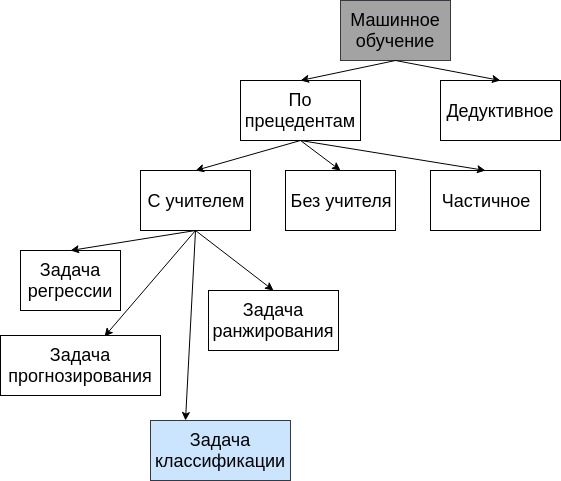
\includegraphics[width=.9\textwidth]{img/ml}
    \vspace*{6pt}
    \caption{Машинное обучение}\label{fig:project-tree}
  \end{figure}

На рисунке 1.1 представлено дерево способов и задач, которые решаются машинным обучением. Дерево неполное, так как существует очень много способов машинного обучения. Поэтому на данном рисунке показана основная ветвь, имеющая прямое отношение к данному исследованию.

\textbf{Классификатором} называется отображение $\widehat{c}: \mathcal{X} \to \mathcal{C}$, где 
\
$\mathcal{C} = \{C_{1}, C_{2}, \dots, C_{k}\}$ — конечное множество меток классов. Под $C_{i}$ можно также понимать множество объектов, которые относятся к классу с номером $i$. Знак "крышки" означает, что $\widehat{c}(x)$ — оценка истинной, но неизвестной функции $c(x)$. Обучающие примеры для классификатора имеют вид пар $(x,c(x))$, где $x \in \mathcal{X}$ — объект, а $c(x)$ — истинный класс, к которому принадлежит этот объект. Под обучением классификатора понимается выявление функции $\widehat{c}$, которая как можно лучше аппроксимирует $c$ не только на обучающем наборе, но и на всем пространстве объектов.\cite{MLFLACH}

\textbf{Типы классификации:}
\begin{itemize}
  \item Бинарная классификация – требуется определить к какому из двух классов относится объект, простой в техническом отношении случай, который служит основой для решения более сложных задач;
  \item Многоклассовая классификация – множества ответов содержит больше двух классов, задача классификации становится более трудной, разделение не так очевидно, как в первом случае. Обычно реашиется с помощью разбиения на более простые подзадачи и сводится к бинарной классификации;
  \item Непересекающиеся классы – объект относится только к одному из множества классов;
  \item Пересекающиеся классы – объект может относиться одновременно к нескольким классам;
  \item Нечёткие классы – определяется степень принадлежности объекта каждому из классов.
\end{itemize}

\textbf{Типы входных данных:}
\begin{itemize}
  \item Признаковое описание — каждый объект – это набор признаков, признаки могут быть числовыми или нечисловыми;
  \item Матрица расстояний между объектами. Каждый объект описывается расстояниями до всех остальных объектов обучающей выборки. С этим типом входных данных работают методы ближайших соседей, парзеновского окна, потенциальных функций;
  \item Временной ряд или сигнал, представляет собой последовательность измерений во времени;
  \item Изображение или видеоряд.
\end{itemize}

Также входные данные могут представляться в виде графов, текстов. Они приводятся к первому или второму типу путём предварительной обработки данных и извлечения признаков.

Классификация текстов (документов) — одна из задач информационного поиска, заключающаяся в определении принадлежности текста к одному из нескольких классов на основании содержания текста. Классификацию документов можно организовать с помощью методов машинного обучения. При таком подходе сохраняется необходимость разметки обучающего множества, то есть человек заранее связывает некоторые документы с классами, тем самым формируя обучающий корпус. Таким образом, классификация документов является примером обучения с учителем, в роли учителя выступает человек, размечающий тексты. 

\textbf{Этапы обработки:}
\begin{itemize}
  \item Индексация документов. Переход к числовой модели, преобразование документов в вектора и определение весов слов;
  \item Построение и обучение классификатора. Могут использоваться различные методы машинного обучения: решающие деревья, наивный байесовский классификатор, нейронные сети, метод опорных векторов и др.;
  \item Оценка качества классификации.
\end{itemize}

\newpage
\subsection{Подготовка данных и извлечение признаков}
\

В рамках данной работы речь идет о классификации текстов или документов. Документы, которые требуется классифицировать, – названия моделей конкурента, а множество классов – это множество названий моделей владельца магазина. Входные данные в обучающем корпусе являются текстами, которые необходимо преобразовать и представить в виде, в котором на них сможет обучаться выбранная модель. С использованием всех объектов-документов в наборе обучающих данных составляется словарь размера $n$ - множество всех признаков, встретившихся в документах. Процесс выделения из текстов признаков с использованием разделителя называется токенизацией. 

Далее каждый документ представляется вектором размера $n$, в котором каждому признаку из словаря ставится в соответствие количество вхождений данного признака в документ.

После преобразования текстовых документов к векторам происходит переход к частотности. TF (term frequency — частота слова) — отношение числа вхождений некоторого слова к общему числу слов документа. Оценивается важность слова $t_{i}$ в пределах отдельного документа.

\begin{align} 
tf(t, d) = \frac{n_{t}}{\sum_{k}n_{k}}, \normalsize
\end{align}

где $n_{t}$ — число вхождений слова $t$ в документ, а в знаменателе общее количество слов в документе.

\

IDF (inverse document frequency — обратная частота документа) — инверсия частоты, с которой некоторое слово встречается во всех документах корпуса данных. Таким образом, чем чаще слово встречается в пределах всех коллекции, тем меньше становится вес таких слов. Для каждого слова существует только одно значение IDF в пределах коллекции.

\begin{align} 
idf(t, D) = \log\frac{|\:D\:|}{| \{ \: d_{i} \: \in \: D \: | \: t \in \: d_{i} \: \}| \:},
\end{align}

где $|\:D\:|$ — общее число документов в обучающем корпусе, а в знаменателе логарифма число документов, в которых встречается $t$.

\begin{align} 
tf\-idf(t, D) = tf(t, d) \times idf(t, D)
\end{align}

Мера TF-IDF это произведение TF и IDF. После нормализации наибольший вес получат слова, которые часто встречаются в пределах какого-либо документа, но редко во всей коллекции документов. 

\newpage
\subsection{Машина опорных векторов}
\

Существует множество алгоритмов, которые используются для обучения текстовых классификаторов. Одним из них является метод опорных векторов, выбранный мной в соответстивии с реультатами исследования, проведенными Т. В. Батурой в статье "Методы автоматической классификации текстов".\cite{TEXTCLASSIFICATION} В этой статье проводится сравнение нескольких алгоритмов и выявляется, что одно из лучших соотношений характеристик качества достигается при использовании метода опорных векторов (для коллекция текстов объемом 1 000–2 000 текстов точность 80–85 \%, полнота 83–87 \%).

\

  \begin{figure}[h!]
    \centering
    \setlength{\fboxsep}{5pt}
    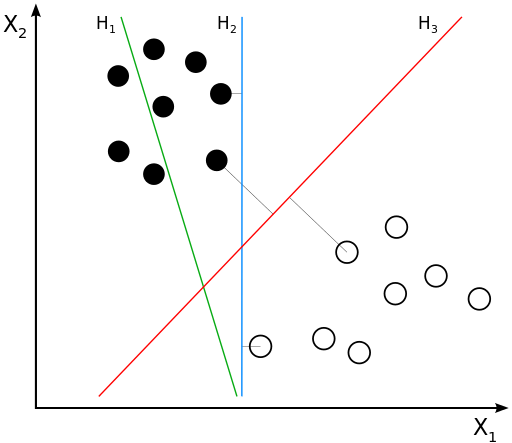
\includegraphics[width=.9\textwidth]{img/svm}
    \vspace*{6pt}
    \caption{Метод опоных векторов}\label{fig:project-tree}
  \end{figure}

\

Машина опорных векторов (метод опорных векторов) – это модель на основе обучения с учителем. Существует множество векторов размера $n$. Каждый из них представляется точкой в $n$-мерном пространстве. Основная задача состоит в том, чтобы найти гиперплоскость размерности $(n-1)$, которая сможет разделить точки в указанном пространстве, тем самым обозначая их принадлежность к разным классам. Причем расстоние от ближайших к гиперплоскости точек до самой гиперплоскости, которое называется зазором, должно быть максимальным, так как предполагается, что это обеспечит наибольшую точность при классификации. В случае линейной неразделимости, то есть когда невозможно найти гиперплоскость, разделяющую множество точек, все вектора переводятся в пространство более высокой размерности и определяется разделяющая гиперплоскость.\cite{Vyugin}

В случае мультиклассовой классификации применяется решающее правило, основанное на разбиении задачи на бинарные по схеме "один против остальных" (one-vs-rest). Обучается n классификаторов, где n – количество классов. Классификатор с самым высоким значением функции выхода используется при классификации.

На рисунке 1.2 показано множество векторов, изображенных в виде точек, и несколько гиперплоскостей, разделяющих эти точки на два класса. Точки, ближайшие к гиперплоскостям, называются опорными векторами. По расстоянию от гиперплоскости до опорных векторов (перпендикуляр изображен серым цветом) определяется величина зазора. На рисунке оптимальной гиперплоскостью является $H_{3}$, так как зазор является максимальным.

Изначально алгоритм построения оптимальной разделяющей гиперплоскости являлся алгоритмом линейной классификации. Однако позднее был предложен способ создания нелинейного классификатора, в основе которого лежит переход от скалярных произведений к произвольным ядрам, kernel trick, позволяющий строить нелинейные разделители. Результирующий алгоритм похож на алгоритм линейной классификации, но скалярное произведение заменяется нелинейной функцией ядра (скалярным произведением в пространстве с большей размерностью). В этом пространстве уже может существовать оптимальная разделяющая гиперплоскость. Так как размерность получаемого пространства может быть больше размерности исходного, то преобразование, сопоставляющее скалярные произведения, будет нелинейным, а значит функция, соответствующая в исходном пространстве оптимальной разделяющей гиперплоскости, будет также нелинейной.

\newpage
\subsection{Анализ имеющихся решений}
\

Одним из имеющихся решений является Elasticsearch. \textbf{Elasticsearch} - свободная программная поисковая система, написанная на языке Java, которая используется большим числом крупных сайтов и компаний, например, GitHub, Foursquare, SoundCloud и другие. Данная система может использоваться для решений многих задач, одной из которых является сопоставление товаров для систем мониторинга цен конкурентов.\cite{ELASTIC} Однако для организации связей товаров Elasticsearch требует четкого задания классов синонимов, то есть групп слов, которые будут распознаваться как один и тот же признак в названии товара. Такой способ не подходит, если в поиске участвует большой объем названий товаров из разных категорий и невозможно вручную установить связи между словами из-за их количества и неопределенности.

\newpage
\subsection{Постановка задач исследования}
В рамках данной работы поставлена задача разработать программу, которая сможет находить связи между товарами, основываясь на предсказаниях обученного на корпусе данных классификатора.
Для решения поставленной цели необходимо решить следующие задачи:
\begin{itemize}
  \item Определить требования к программе;
  \item Спроектировать архитектуру программы;
  \item Реализовать программу в соответствии с разработанной архитектурой;
  \item Провеси тестирование.
\end{itemize}
\newpage
